\section{Testing  Platform}\label{sec:testing_platform}
\subsection{Hardware}
The basis of the designed test platform is HopeRF's\footnote{HopeRF Microelectronics Co. Ltd, China, https://www.hoperf.com/} RFM95W - a packet radio containing a \ac{lora} transceiver design licensed from Semtech; specifically, a broken out version from  Adafruit's\footnote{Adafruit, USA, https://www.adafruit.com/} is used. As a raw packet radio, unlike the popular Microchip RN2483, it provides direct access to the radio interface. An omni-directional 3dBi gain half-wavelength whip antenna is connected to the radio using a soldered uFL connector and a SMA to uFL connector. It is controlled by a Teensy\footnote{Teensy, https://www.pjrc.com/teensy/} 3.6 micro-controller, which also handles all logging responsibilities. A simple breakout circuit is implemented on strip-board to connect the components in a condensed package. Each breakout board features: a JST-PH2 battery connector, a coin cell holder for the Teensy's real-time-clock (\ac{rtc}), a power switch, a two-mode software switch, and three status LEDs. The schematic can be viewed in Figure \ref{fig:datalogger_schematic}. This is packaged to fit in an IP67 rated container with an internal 1800mAh \ac{lipo} battery. Switches and SMA antenna connectors are external; these are IP67 rated and sealant is added where appropriate. The Teensy is equipped with an SD card for storage but, due to cost considerations, a GPS module is not implemented. A full breakdown of materials is listed in Figure \ref{fig:datalogger_cost}. The created test platforms, seen in Figure \ref{fig:dataloggers}, achieve the target of being a \ac{lora} datalogger suitable for all-weather.

\begin{figure}[H]
    \centering
    \begin{tabular}{cc}
    \subfloat[]{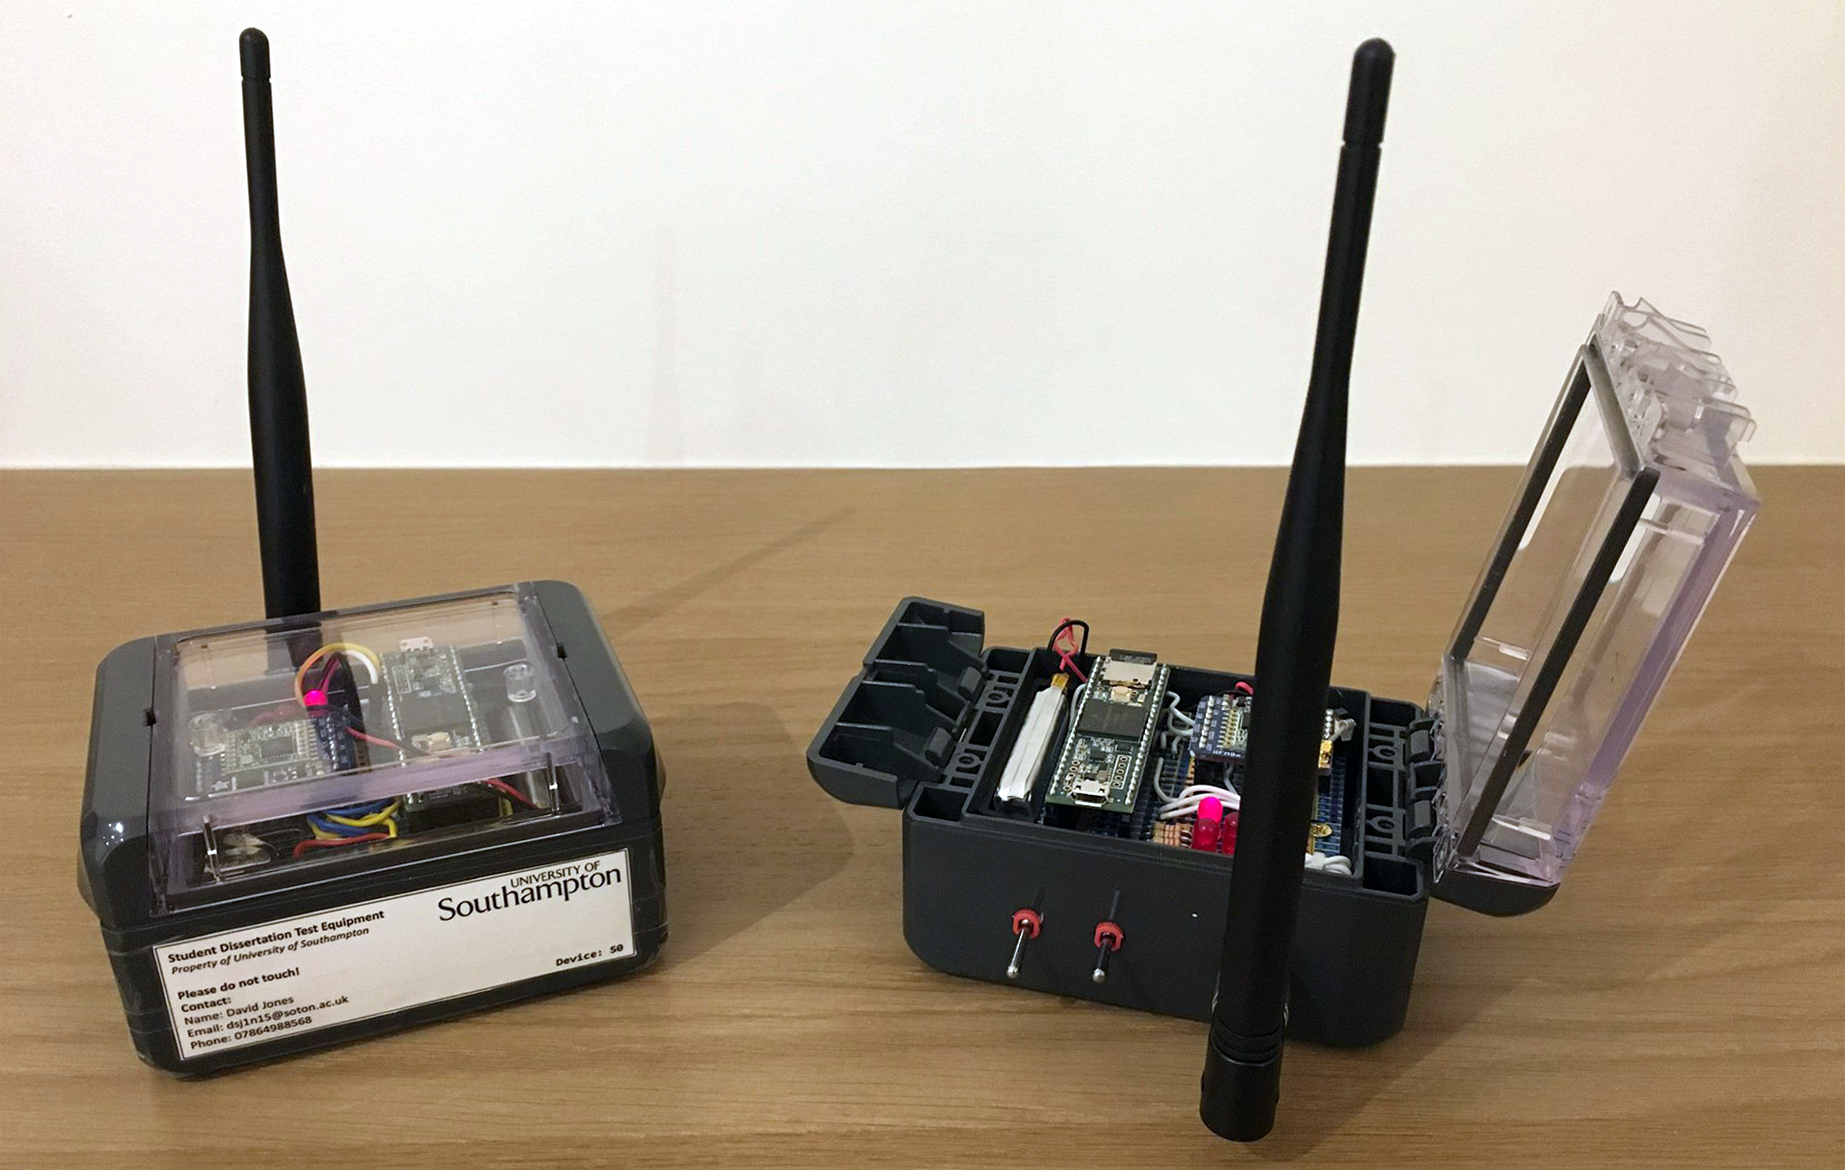
\includegraphics[height=5cm]{Figures/dl_both_devices.png}}
    \hspace{2.5mm}
    \subfloat[]{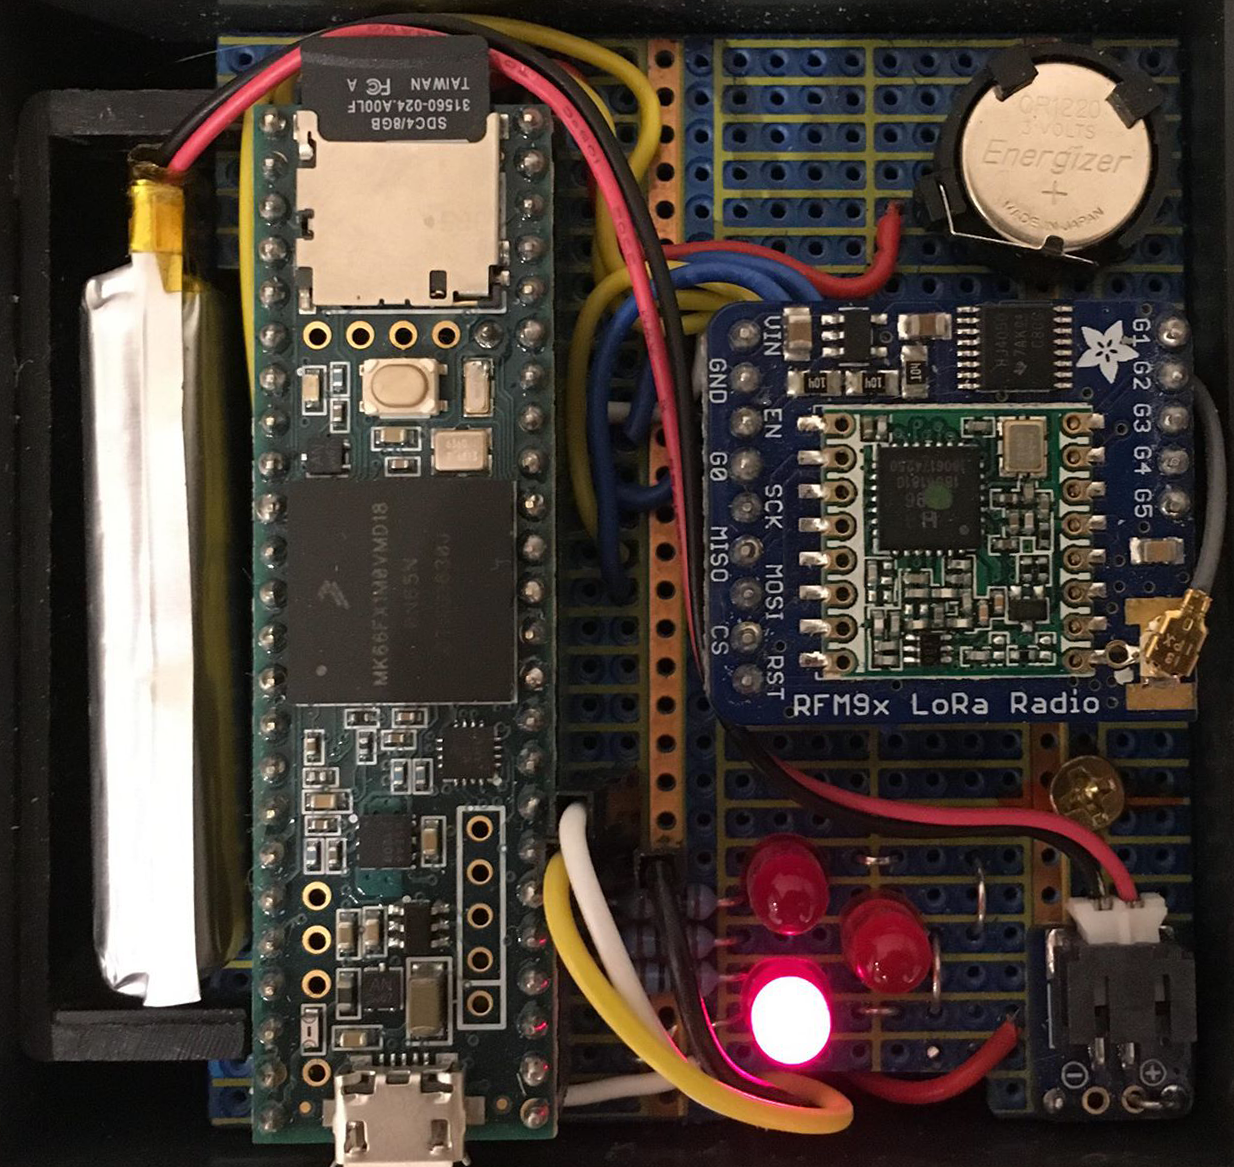
\includegraphics[height=5cm]{Figures/dl_circuit.png}}
    \end{tabular}
    \caption[Assembled testing platform]{External view of \texttt{S0} and \texttt{M0} platforms (left). Circuit view of \texttt{S0} (right); this is fixed into the assembly to avoid movement between tests. }
    \label{fig:dataloggers}
\end{figure}

\subsection{Software}\label{sec:test_platform_software}
The system is designed such that one device (a slave), can be left unattended at a fixed location and controlled by a second device (a master); this is achieved using a command control system, as explained in Figure \ref{fig:software_cmd_system}. Two command classes are defined for testing purposes; these are as follows:
\begin{itemize}
	\item {\textbf{\texttt{HB\_CMD}}} : Command to trigger simple heartbeat functionality. When a slave receives this command it sends a heartbeat response (\textbf{\texttt{HB\_RSP}}) on the base configuration.
	\item {\textbf{\texttt{TD\_CMD}}} : Command to trigger execution of a test definition (\ac{td}). A \ac{td} holds a \ac{lora} configuration (values for \ac{cf}, \ac{sf}, \ac{tp}, \ac{bw}, \ac{cr}, \ac{pl}), a required \ac{pc}, and packet length. Figure \ref{fig:software_testdef_execution} explains full control flow in detail.
	\end{itemize}
	
\begin{figure}[H]
    \centering
    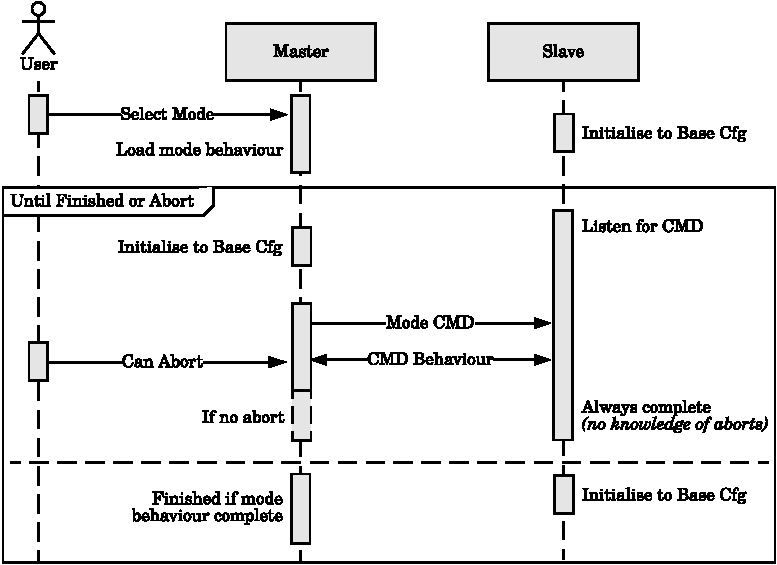
\includegraphics{Figures/software_cmd_system.pdf}
    \caption[Master-Slave command control method]{
    	Diagram showing master-slave command control method. Initially, both devices default to the same hardcoded radio parameters allowing two-way communication. This base state is chosen such that the expected range exceeds or matches that of the longest test range. When a mode is selected on the master, it sends the corresponding command to the listening slave and the behaviour is carried out. At any point the user may stop the master, and unless the slave is interacting with the master, it likely has no knowledge of this and will finish its behaviour. After command behaviour has finished the base configuration is reloaded in case it has been changed. In the case a master's mode requires multiple commands, the process repeats.
    }
    \label{fig:software_cmd_system}
\end{figure}
\vspace{-0mm}
Slaves always listen to handle incoming commands, whereas the master can be set into two modes (other than idle):
\begin{itemize}
	\item \textbf{Heartbeat:} Sends periodic \texttt{HB\_CMD} commands, alerts user accordingly for every received or missed \textbf{\texttt{HB\_RSP}}.
	\item {\textbf{Run \ac{td}s:} Loads all stored \ac{td}s and handles them sequentially using \textbf{\texttt{TD\_CMD}}s. \ac{td} results are stored separately in a folder timestamped with the execution time.}
\end{itemize}

Interfacing with the radio is handled by the RH\_RF95 driver from the Radiohead\footnote{Radiohead, https://www.airspayce.com/mikem/arduino/RadioHead/} library; this means that only the control logic needed to be implemented. Operation of the software is detailed in Appendix \ref{sec:user_manual}.

\begin{figure}[H]
    \centering
    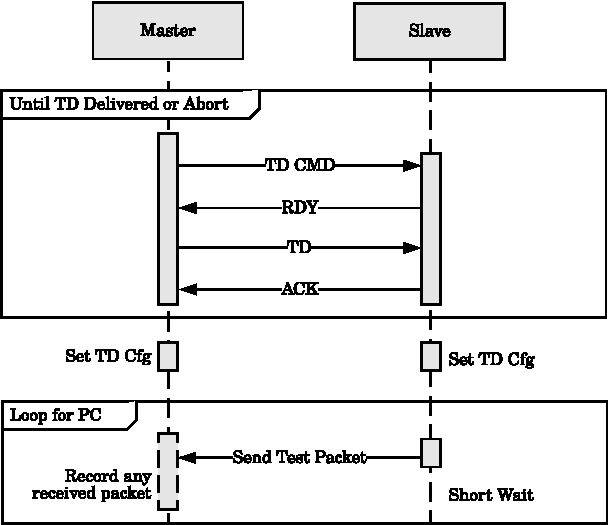
\includegraphics{Figures/software_testdef_execution.pdf}
    \caption[Master-Slave test definition execution method]{
    	Diagram showing execution of a single \ac{td}. After a \textbf{\texttt{TD\_CMD}} command is received, a short handshake takes place so that the master can share the \ac{td} to execute. After which both radios accordingly change their parameters and the slave sends the required \ac{pc}. Test packets are of length defined by the \ac{td} and contain a sequence identifier with the rest of data filled by a fixed data pattern. Any received packets are recorded along with \ac{rssi} and \ac{snr} values. Failed receives that occur due to bad CRCs are also recorded. This means that only transmissions where the preamble is not received are not recorded.
    }
    \label{fig:software_testdef_execution}
\end{figure}